\documentclass[paper=a4, fontsize=11pt]{jhwhw} % A4 paper and 11pt font size
\usepackage{pgfplots}
\pgfplotsset{compat=1.9}
\usepackage{amsmath, amssymb}
\newcommand\SetSymbol[1][]{\:#1\vert\:}
\providecommand\given{} % to make it exist
\DeclarePairedDelimiterX\Set[1]\{\}{\renewcommand\given{\SetSymbol[\delimsize]}#1}
\usepackage{listings}
\usepackage{color}

\definecolor{dkgreen}{rgb}{0,0.6,0}
\definecolor{gray}{rgb}{0.5,0.5,0.5}
\definecolor{mauve}{rgb}{0.58,0,0.82}

\lstset{frame=tb,
  language=Python,
  aboveskip=3mm,
  belowskip=3mm,
  showstringspaces=false,
  columns=flexible,
  basicstyle={\small\ttfamily},
  numbers=none,
  numberstyle=\tiny\color{gray},
  keywordstyle=\color{blue},
  commentstyle=\color{dkgreen},
  stringstyle=\color{mauve},
  breaklines=true,
  breakatwhitespace=true,
  tabsize=3
}
\begin{document}
\title{Discrete Math - Homework Set \#7}
\author{Ben Haines (bmh5wx)}
\problem{\#1}
Define binary relations $R$ and $S$ from $\mathbb R$ to $\mathbb R$ as follows:
$$R = \Set{(x, y)\in \mathbb R \times \mathbb R\given x^2 + y^2 = 4} \text{ and } S = \Set{(x,y)\mathbb R\times \mathbb R\given x = y}.$$
Graph $R, S, R\cup S$, and $R\cap S$ in the Cartesian plane.
\solution
\begin{center}
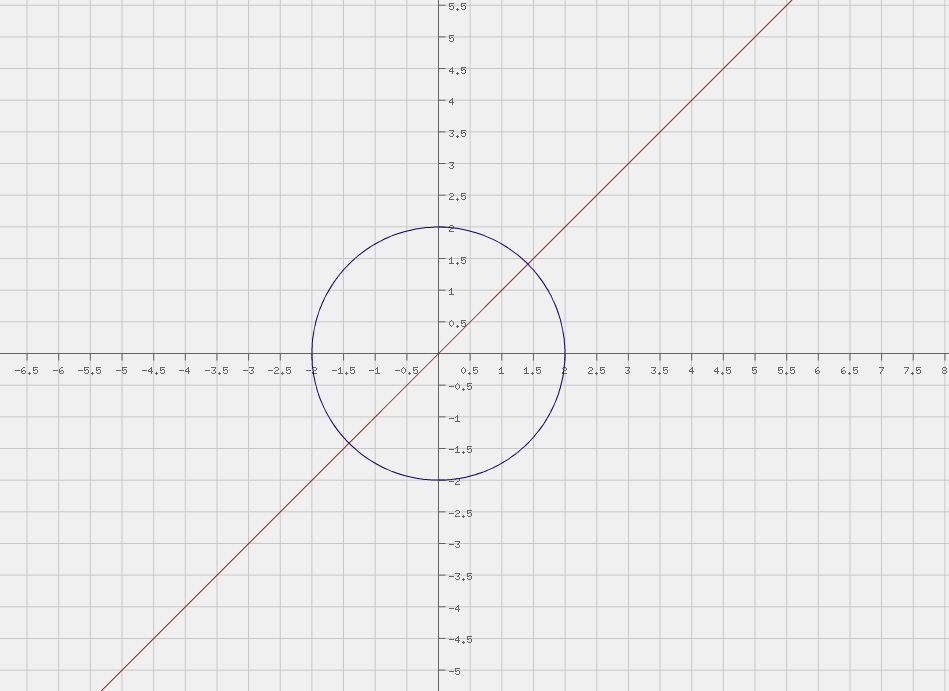
\includegraphics[scale=0.4]{hw7}
\end{center}
In the above graph, $R$ is represented by the blue circle, $S$ is represented by the red line, $R\cup S$ is the line and circle taken together, and $R\cap S$ is the two points of intersection between the line and the circle.
\problem{\#2}
Let $S$ be the set of all strings  $a$'s and $b$'s. Define a relation $T$ on $S$ as follows:
$$\text{For all}, s,t\in S, sTt \iff t = as$$
(that is, $t$ is the concatenation of $a$ with $s$)
\begin{enumerate}
    \item Is $abTaab$?
    \item Is $aabTab$?
    \item Is $baTaba$?
    \item Is $abaT^{-1}ba$?
    \item Is $abbT^{-1}bba$?
    \item Is $abbaT^{-1}bba$?
\end{enumerate}
\solution
\part
Yes.
\part
No. $aabTaaab$.
\part
Yes.
\part
Yes.
\part
No. $abbT^{-1}bb$.
\part
Yes.


\problem{\#3}
Let $A=\Set{2, 4}$ and $B=\Set{6, 8, 10}$ and define relations $R$ and $S$ from $A$ to $B$ as follows:
\begin{align*}
    &R = \Set{(x, y)\given x\in A \text{ and } y\in B \text{ and } x\mid y} && S = \Set{(x,y)\given x\in A \text{ and } y\in B \text{ and } y=x+4}
\end{align*}
State explicitly which ordered pairs are in $A\times B, R, S, R\cup S$, and $R\cap S$.
\solution
$A\times B = \Set{(2, 6), (2, 8), (2, 10), (4, 6), (4, 8), (4, 10)}$,
$R = \Set{(2, 6), (2, 8), (2, 10), (4, 8)}$,
$S = \Set{(2, 6), (4, 8)}$,
$R\cup S = \Set{(2, 6), (2, 8), (2, 10), (4, 8)}$,
$R\cap S = \Set{(2, 6), (4, 8)}$

\problem{\#4}
Suppose that $A=\Set{1, 2, 3}, B=\Set{4, 5, 6}, R=\Set{(1, 4), (1, 6), (2, 6), (3, 5)}, \text{ and }\\ S = \Set{(4, 5), (4, 6), (6, 4), (5, 5)}$. Note that $R$ is a relation from $A$ to $B$ and $S$ is a relation from $B$ to $B$. Find the following relations, showing all work supporting how you found those relations:
\begin{enumerate}
    \item $S\circ R$
    \item $S\circ S^{-1}$
\end{enumerate}
\solution
$A\times B = \Set{(1, 4), (1, 5), (1, 6), (2, 4), (2, 5), (2, 6), (3, 4), (3, 5), (3, 6)}$,\\
$B\times B = \Set{(4, 4), (4, 5), (4, 6), (5, 4), (5, 5), (5, 6), (6, 4), (6, 5), (6, 6)}$
\part
$R \subseteq A\times B$ and $S\subseteq B\times B$. $S\circ R = \Set{(a, b)\in A\times B\given \exists b_2\in B:(a, b_2)\in R \land (b_2, b)\in S}$
Using this as a guide and checking each element of $A\times B$ we find that $R\circ S = \Set{(1, 5), (1, 6), (2, 4), (3, 5)}$.
\part
$S^{-1} = \Set{(5, 4), (6, 4), (4, 6), (5, 5)}$. Then $S\circ S^{-1} = \Set{(a, b)\in B\times B\given \exists c\in B: (a, c)\in S \land (c, a)\in S^{-1}}$. Using this as a guide and checking each element in $B\times B$ we find$S\circ S^{-1} = \Set{(4, 4), (4, 5), (5, 4), (5, 5), (6, 6)}$.

\problem{\#5}
For relation $R$ and its inverse $R^{-1}$:
\begin{enumerate}
    \item What properties \textit{must} hold for relation $R$ if $R = R^{-1}$. Explain.
    \item What properties \textit{might} hold if $R=R^{-1}$. Explain.
\end{enumerate}
\solution
\part
$R = R^{-1}$ is equivalent to saying that $(a, b)\in R \implies (b, a) \in R$. Therefore $R$ must be symmetric.
\part
$R$ might be transitive or reflexive. There is nothing in the statement that $R=R^{-1}$ that makes either of these properties impossible, but neither is there anything that guarantees them.

\problem{\#6}
Determine whether the given relation is an equivalence relation. Justify your answers by showing which properties of an equivalence relation are true and which are not.
\begin{enumerate}
    \item Let $A$ be the set of all lines in the plane. The relation $R$ is defined on $A$ as follows, two lines $X$ and $Y$ relate to one another if they have the same slope.
    \item Let $X$ be a nonempty set and $P(X)$ be the power set of $X$. Define a relation $R$ on subsets of $P(X)$ such that $A$ relates to $B$ if the cardinality of $A$ does not equal the cardinality of $B$.
\end{enumerate}
\solution
\part
This is an equivalence relation. A line must have the same slope as itself so the relation is reflexive. If line $a$ has the same slope as line $b$ then line $b$ has the same slope as line $a$ so the relation is symmetric. If line $a$ has the same slope as line $b$ and line $b$ has the same slope as line $c$ then line $a$ has the same slope as line $c$ so the relation is transitive.
\part
This is not an equivalence relation. A set must have the same cardinality as itself so the relation is not reflexive. If set $A$ has the same cardinality as set $B$ then set $B$ must have the same cardinality as set $A$ so the relation is not symmetric. If set $A$ has the same cardinality as set $B$ and set $B$ has the same cardinality as set $C$ then set $A$ must have the same cardinality as set $C$ so the relation is not transitive.

\problem{\#7}
If $R$ is symmetric and $R$ is transitive then $R$ is reflexive. This can be proven by considering $(x, y)\in R$. By symmetry, $(x, y)\in R \implies (y, x)\in R$. Using transitivity, $(x, x)\in R$, thus $R$ is reflexive. What's wrong with this proof?
\solution
The proof assumes that $R$ contains some element $(x, y)$. Consider the relation $R=\emptyset$ on $\mathbb Z\times \mathbb Z$. $R$ is both transitive and symmetric but it is not reflexive.
\problem{\#8}
Given a set, $A$, where $A=\Set{a[1], a[2], \ldots, a[n]}$ (represented as a one dimensional array) and a relation, $R$, on $A$, design the following (use pseudocode):
\begin{enumerate}
    \item An algorithm to test whether $R$ is reflexive.
    \item An algorithm to test whether $R$ is symmetric.
    \item An algorithm to test whether $R$ is transitive.
\end{enumerate}
\solution
\part
\begin{lstlisting}
for a in A:
    if (a, a) not in R:
        return false
return true
\end{lstlisting}
\part
\begin{lstlisting}
for a in A:
    for b in A:
        if (a, b) in R and (b, a) not in R:
            return false
return true
\end{lstlisting}
\part
\begin{lstlisting}
for a in A:
    for b in A:
        if (a, b) in R:
            for c in A:
                if (b, c) in R:
                    if (a, c) not in R:
                        return false
return true
\end{lstlisting}
  

\problem{\#9}
Prove or disprove the following: (Suppose that $R$ and $S$ are binary relations on a set $A$).
\begin{enumerate}
    \item If $R$ and $S$ are reflexive, then $R\cup S$ is also reflexive.
    \item If $R$ and $S$ are symmetric, then $R\cup S$ is also symmetric.
\end{enumerate}
\solution
\part
Take any element $a$ of $A$. The relation $R$ is reflexive so therefore $(a, a)\in R$. By the definition of set unions $(a, a)\in R\cup S$ for all $a\in A$ so $R\cup S$ is reflexive.
\part
Select any element $(a, b)\in R\cup S$. By the definition of set unions $(a, b)$ is either an element of $R$ or of $S$. If it's an element of $R$ then we know that $(b, a)\in R$ because $R$ is reflexive and therefore $(b, a)\in R\cup S$. Similarly, if $(a, b)\in S$ we know that $(b, a)\in S$ because $S$ is symmetric and therefore $(b, a)\in R\cup S$. In every case, $(a, b)\in R\cup S \implies (b,a)\in R\cup S$ and therefore $R\cup S$ is symmetric.
\end{document}
